\documentclass{article}
\usepackage{pgffor, siunitx}
\usepackage{import}
\usepackage{graphicx} % Allows image inclusion
\usepackage{wrapfig}
\usepackage{float}
\usepackage{svg}
\usepackage[hidelinks]{hyperref}
\usepackage{tikz}
\usetikzlibrary{arrows.meta}
\usetikzlibrary{calc}
\usetikzlibrary{matrix}

% Matematik
\usepackage{amssymb}  % most common
\usepackage{amsmath, mathrsfs, pgfmath}

\usepackage{ifthen}

% Værktøjer
% Til at folde lister ud med 
\newcounter{vaerdiet}
\newcounter{vaerdito}                           % Numerisk 
\newcounter{vaerditre}
\newcounter{vaerdifire}
\newcommand{\vaerdifem}{-\infty}
\newcommand{\vaerdiseks}{\infty}                % Symbolsk
\newcommand{\vaerdisyv}{-\infty}
\newcommand{\vaerdiotte}{\infty}                

\def\register#1#2{\registerAllokering#2\nil{#1}}
\def\registerAllokering#1,#2\nil#3{
    \ifcase#3                                   % Register 1 ( Numerisk)
        \setcounter{vaerdiet}{#2}
        \setcounter{vaerdito}{#1}
    \or                                         % Register 2 ( Numerisk)
        \setcounter{vaerditre}{#2}
        \setcounter{vaerdifire}{#1}
    \or                                         % Register 3 ( Symbols)
        \edef\vaerdifem{#2}                
        \edef\vaerdiseks{#1}
    \or 
        \edef\vaerdisyv{#2}                
        \edef\vaerdiotte{#1}
    \else
        %   
    \fi
}
\def\registeret#1,#2\nil{%
    \setcounter{vaerdiet}{#1}
    \setcounter{vaerdito}{#2}
}%
\def\registerto#1,#2\nil{%
    \setcounter{vaerditre}{#1}
    \setcounter{vaerdifire}{#2}
}%
\def\registertre#1,#2\nil{%                     % Symbolsk register
    \edef\vaerdifem{#1}                
    \edef\vaerdiseks{#2}
}%
\def\registerfire#1,#2\nil{%                     % Symbolsk register
    \edef\vaerdisyv{#1}                
    \edef\vaerdiotte{#2}
}%
\newcommand{\udfold}[2]{
    \ifnum#1=1
        % \registeret#2\nil
        \registerto#2\nil           % Numerisk
    \else
        \ifnum#1=0
            \registeret#2\nil       % Numerisk
        \else   
            \ifnum#1=2
                \registertre#2\nil  % Symbolsk 
            \else
                \registerfire#2\nil % Symbolsk 
            \fi
        \fi
    \fi
}

% Tekst redigering 
\newcommand{\tab}{\quad}
\newcommand{\transformation}[1]{\tab\overset{\mathscr{#1}}{\leftrightarrow}\tab}

% Counters 
\newcounter{kapitel}
\newcounter{alfabetTabular}
\renewcommand{\thealfabetTabular}{\alph{alfabetTabular}}

% Kapitel Context 
\newenvironment{kapitel}[1][]{
    \clearpage
    \refstepcounter{kapitel} % Increment counter first
    \subsection*{Kapitel \thekapitel: #1}
}{}

% Formelsamling / Opgaver / Øvelser mm...
\newenvironment{rubrik}[1][]{
    \clearpage
    \section*{#1}
    \setcounter{kapitel}{0} % Nulstil counteren, I tilfælde af, at den har været brugt. 
}{}

\newenvironment{underrubrik}[1][]{
    \subsection*{#1}
}{}

% Indhold
\newenvironment{Formelsamling}{\begin{rubrik}[Formelsamling]\end{rubrik}}{}
\newenvironment{Udledninger}{\begin{rubrik}[Udledninger]\end{rubrik}}{}

\newenvironment{Opgaver}{\begin{rubrik}[Opgaver]\end{rubrik}}{}
\newenvironment{Opgave}[1][]{\begin{underrubrik}[#1]\end{underrubrik}\setcounter{alfabetTabular}{0}}{\vspace{100pt}}
\newenvironment{UnderOpgave}[1][]{
    \refstepcounter{alfabetTabular}
    \subsubsection*{\boldmath{\thealfabetTabular. #1}}}{}

\newenvironment{Øvelser}{\begin{rubrik}[Øvelser]\end{rubrik}}{}
\newenvironment{Øvelse}[1][]{\begin{underrubrik}[#1]\end{underrubrik}}{}

\newenvironment{Udklip}{\color{red}\begin{rubrik}\end{rubrik}}{}              % Skal bruges til når jeg retter opgaver, så fletter jeg de forkerte ind i det her. 

\newcommand{\filterZ}[2]{
    \frac{
        \foreach \b [count=\j from 0] in {#1} {
            \ifnum\j=0
                \b
            \else
                \pgfmathparse{ifthenelse(\b<0, "", "+")}\pgfmathresult \b z^{-\i}
                % + \b z^{-\the\numexpr\j-1}
            \fi
        }% 
    }{
        \foreach \a [count=\i from 0] in {#2} {
            \ifnum\i=0
                \a
            \else
                \pgfmathparse{ifthenelse(\a<0, "", "+")}\pgfmathresult \a z^{-\i}
                % + \a z^{-\the\numexpr\i-1}
            \fi
        }
    }
}
\newcommand{\cosTilEksponentiel}[1]{ \frac{e^{j#1} + e^{-j#1}}{2} }
\newcommand{\sinTilEksponentiel}[1]{ \frac{e^{j#1} - e^{-j#1}}{2j} }
\newcommand{\lavKolonneData}[3]{  
    % Store in the column variables (c1, c2, c3,...)
    \expandafter\xdef\csname c1\the\numexpr\value{raekketaeller}+1\endcsname{#1}  
    \expandafter\xdef\csname c2\the\numexpr\value{raekketaeller}+1\endcsname{#2}  
    \expandafter\xdef\csname c3\the\numexpr\value{raekketaeller}+1\endcsname{#3}  
    
    % Increment the column counter for the next column
    \stepcounter{raekketaeller}  
}
% Set up a counter to keep track of the column number
\newcounter{raekketaeller}\setcounter{raekketaeller}{0}


\NewDocumentEnvironment{EgenTabel}{+b}{
    % ------- Lav dataen -------
    #1 
}{
    % ------- Vis dataen -------
    \vspace{10pt}
    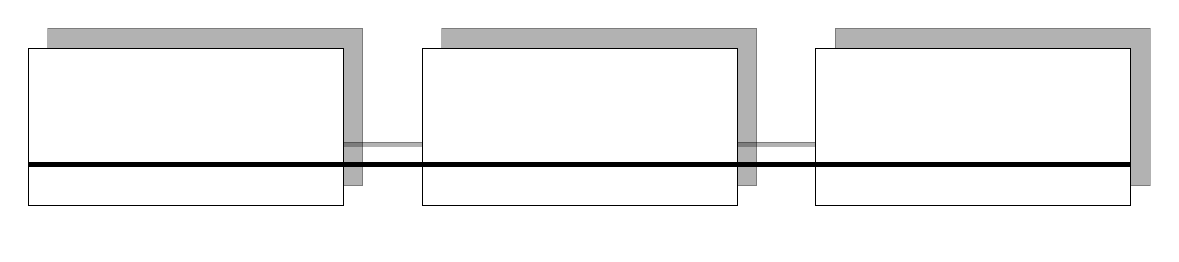
\begin{tikzpicture}
        \tikzset{
            shadow/.style={fill=black, opacity=0.3},        % Skygge 
            cell/.style={fill=white, draw=black, very thin}, % Celle 
        }
        % Baggrund of celler
        \filldraw[shadow] (0.25, 0.5*\theraekketaeller + 2 + 0.25 - 1.5) rectangle(12, 0.5*\theraekketaeller + 2 + 0.25 - 1.5 + 0.05);
        \foreach \x in {0, ..., 2} {
            \filldraw[shadow] (\x*5 + 0.25, 0.25) rectangle(\x*5 + 4.25, 0.5*\theraekketaeller + 2 + 0.25); 
            \filldraw[cell] (\x*5, 0) rectangle(\x*5 + 4, 0.5*\theraekketaeller + 2); 
        }
        % Visning af data.
        \foreach \i in {1, 2, ..., \theraekketaeller} {
            \ifnum\i=1
                \filldraw[black] (0.5, 0.5*\theraekketaeller + 2 - 0.75) node[anchor=west] {$\csname c1\i\endcsname$};
                \filldraw[black] (5.5, 0.5*\theraekketaeller + 2 - 0.75) node[anchor=west] {$\csname c2\i\endcsname$};                
                \filldraw[black] (10.5,0.5*\theraekketaeller + 2 - 0.75) node[anchor=west] {$\csname c3\i\endcsname$};
            \else
                \filldraw[black] (0.5, 0.5*\theraekketaeller + 2 - 1.25 - 0.5*\i) node[anchor=west]{$\csname c1\i\endcsname$};
                \filldraw[black] (5.5, 0.5*\theraekketaeller + 2 - 1.25 - 0.5*\i) node[anchor=west]{$\csname c2\i\endcsname$};
                \filldraw[black] (10.5, 0.5*\theraekketaeller + 2 - 1.25 - 0.5*\i) node[anchor=west]{$\csname c3\i\endcsname$};
            \fi
        }
        % Horinsontal linje. 
        \filldraw[black] (0, 0.5*\theraekketaeller + 2 - 1.5) rectangle(14, 0.5*\theraekketaeller + 2 - 1.5 + 0.05);
    \end{tikzpicture}\setcounter{raekketaeller}{0}
}








% Indhold
\graphicspath{{Indhold/Billeder/}}
% Indstillinger: 
% Billednr:109

\newcommand{\fetchBillede}[2]{\includegraphics[scale=#2]{#1}}
\newcommand{\fetchSVG}[2]{\includesvg[scale=#2]{#1}} % width=1.0\textwidth
\newcommand{\fig}[2]{
    \begin{figure}[h!]
        % \centering
        % \top
        \makebox[\textwidth]{
            \fetchBillede{#1}{#2}
        }
        \caption{#1}
        \label{fig:#1}
    \end{figure}
}



\newcommand{\figSVG}[2]{
    \begin{figure}[h!]
        \centering
        \makebox[\textwidth]{
            \fetchSVG{#1}{#2}
        }
        \caption{#1}
        \label{fig:#1}
    \end{figure}
}


% \figen{0.2} => scaling = 0.2
\newcommand{\figen}[1]{\fig{Z transformations egenskaber}{#1}}
\newcommand{\figto}[1]{\fig{Blokdiagram kapitel 2.png}{#1}}
\newcommand{\figtre}[1]{\figSVG{Feedback system.svg}{#1}}
\newcommand{\figfire}[1]{\fig{Opgave 2.1.png}{#1}}
\newcommand{\figfem}[1]{\fig{Opgave 2.3.png}{#1}}
\newcommand{\figseks}[1]{\fig{Opgave 2.5.png}{#1}}
\newcommand{\figsyv}[1]{\fig{Opgave til kapitel 2.png}{#1}}
\newcommand{\figotte}[1]{\fig{Opgave 2.17.a.png}{#1}}
\newcommand{\figni}[1]{\fig{Opgave 2.17.b.png}{#1}}
\newcommand{\figti}[1]{\fig{Opgave 2.17.c.png}{#1}}
\newcommand{\figeleve}[1]{\fig{Opgave 2.17.png}{#1}}
\newcommand{\figtolv}[1]{\fig{Opgave 2.33.png}{#1}}
\newcommand{\figtretten}[1]{\figSVG{Opgave 2.50.svg}{#1}}
\newcommand{\figfjorten}[1]{\fig{Opgave 2.50.png}{#1}}
\newcommand{\figfemten}[1]{\fig{Opgave 3.1.a.png}{#1}}
\newcommand{\figseksten}[1]{\fig{Opgave 3.1.b.png}{#1}}
\newcommand{\figsytten}[1]{\fig{Opgave 3.1.d.png}{#1}}
\newcommand{\figatten}[1]{\fig{SløretBillede.png}{#1}}
\newcommand{\fignitten}[1]{\fig{AfsløretBillede.png}{#1}}
\newcommand{\figtyve}[1]{\fig{AfsløretsFilter.png}{#1}}
\newcommand{\figenogtyve}[1]{\fig{Opgave 3.15.png}{#1}}
\newcommand{\figtoogtyve}[1]{\fig{Opgave 3.16.png}{#1}}
\newcommand{\figtreogtyve}[1]{\fig{Opgave 3.19 - pzmap.png}{#1}}
\newcommand{\figfireogtyve}[1]{\fig{Opgave 3.19 - Respons.png}{#1}}
\newcommand{\figfemogtyve}[1]{\fig{Opgave 5.2.png}{#1}}
\newcommand{\figseksogtyve}[1]{\fig{Opgave 5.2.e.png}{#1}}
\newcommand{\figsyvogtyve}[1]{\fig{Opgave 5.30.png}{#1}}
\newcommand{\figotteogtyve}[1]{\fig{Opgave 5.48.png}{#1}}
\newcommand{\figniogtyve}[1]{\fig{Opgave 5.48.2.png}{#1}}
\newcommand{\figtredive}[1]{\fig{EKGdata.png}{#1}}
\newcommand{\figenogtredive}[1]{\fig{EKGfrekvenspektrum.png}{#1}}
\newcommand{\figtoogtredive}[1]{\fig{EKGnotchfilterAnalyse.png}{#1}}
\newcommand{\figtreogtredive}[1]{\fig{EKGnotchfilterPZmap.png}{#1}}
\newcommand{\figfireogtredive}[1]{\fig{EKGsignalfiltreret.png}{#1}}
\newcommand{\figfemogtredive}[1]{\fig{EKGforbedretNotchfilterAnalyse.png}{#1}}
\newcommand{\figseksogtredive}[1]{\fig{EKGforbedretNotchfilterPZmap.png}{#1}}
\newcommand{\figsyvogtredive}[1]{\fig{EKGforbedretSignalFiltrering.png}{#1}}
\newcommand{\figotteogtredive}[1]{\fig{SignalbehandlingTemperaturdata.png}{#1}}
\newcommand{\figniogtredive}[1]{\fig{SignalbehandlingTemperaturdataFiltreret.png}{#1}}
\newcommand{\figfyrre}[1]{\fig{SignalbehandlingTemperaturdataFilteranalyse.png}{#1}}
\newcommand{\figenogfyrre}[1]{\fig{SignalbehandlingTemperaturdataIIRFiltermodFIRFilter.png}{#1}}
\newcommand{\figtoogfyrre}[1]{\fig{Signalbehandling3DAudioelev50H50e096a.png}{#1}}
\newcommand{\figtreogfyrre}[1]{\fig{FilterStabilitet.png}{#1}}
\newcommand{\figfireogfyrre}[1]{\fig{Opgave 5.16.png}{#1}}
\newcommand{\figfemogfyrre}[1]{\fig{Opgave 5.31b.png}{#1}}
\newcommand{\figseksogfyrre}[1]{\fig{Opgave 5.31c.png}{#1}}
\newcommand{\figsyvogfyrre}[1]{\fig{Opgave 5.38.b.png}{#1}}
\newcommand{\figotteogfyrre}[1]{\fig{Opgave 5.38.c.png}{#1}}
\newcommand{\figniogfyrre}[1]{\fig{Opgave 5.55.a.png}{#1}}
\newcommand{\fighalvtreds}[1]{\fig{Opgave 5.55.b.png}{#1}}
\newcommand{\figenoghalvtreds}[1]{\fig{Opgave 5.55.c.png}{#1}}
\newcommand{\figtooghalvtreds}[1]{\fig{Opgave 5.55.d.png}{#1}}
\newcommand{\figtreoghalvtreds}[1]{\fig{Opgave 5.39.a.png}{#1}}
\newcommand{\figfireoghalvtreds}[1]{\fig{Opgave 5.39.b.png}{#1}}
\newcommand{\figfemoghalvtreds}[1]{\fig{Opgave 5.39.c.png}{#1}}
\newcommand{\figseksoghalvtreds}[1]{\fig{Opgave 5.39.d.png}{#1}}
\newcommand{\figsyvoghalvtreds}[1]{\fig{Opgave 6.2.a.png}{#1}}
\newcommand{\figotteoghalvtreds}[1]{\fig{Opgave 6.2.b.png}{#1}}
\newcommand{\fignioghalvtreds}[1]{\fig{Opgave 6.2.c.png}{#1}}
\newcommand{\figtres}[1]{\fig{Opgave 6.12.png}{#1}}
\newcommand{\figenogtres}[1]{\fig{Opgave 6.12.Rekonstruering.png}{#1}}
\newcommand{\figtoogtres}[1]{\fig{Opgave 7.1.png}{#1}}
\newcommand{\figtreogtres}[1]{\fig{Opgave 7.1.c.png}{#1}}
\newcommand{\figfireogtres}[1]{\fig{Opgave 7.3.b.png}{#1}}
\newcommand{\figfemogtres}[1]{\fig{Opgave 7.3.c.png}{#1}}
\newcommand{\figseksogtres}[1]{\fig{Opgave 7.3.d.png}{#1}}
\newcommand{\figsyvogtres}[1]{\fig{Opgave 7.5.png}{#1}}
\newcommand{\figotteogtres}[1]{\fig{Opgave 8. KeyboardMatrix.png}{#1}}
\newcommand{\figniogtres}[1]{\fig{Opgave 8.48.png}{#1}}
\newcommand{\fighalvfjerds}[1]{\fig{Opgave 9.1.png}{#1}}
\newcommand{\figenoghalvfjerds}[1]{\fig{Opgave 9.2.png}{#1}}
\newcommand{\figtooghalvfjerds}[1]{\fig{Opgave 9.3.png}{#1}}
\newcommand{\figtreoghalvfjerds}[1]{\fig{Opgave 9.8.png}{#1}}
\newcommand{\figfireoghalvfjerds}[1]{\fig{Opgave 9.12c.png}{#1}}
\newcommand{\figfemoghalvfjerds}[1]{\fig{Opgave 9.28.png}{#1}}
\newcommand{\figseksoghalvfjerds}[1]{\fig{Opgave 9.29.png}{#1}}
\newcommand{\figsyvoghalvfjerds}[1]{\fig{Eksempel 10.5.a.png}{#1}}
\newcommand{\figotteoghalvfjerds}[1]{\fig{Eksempel 10.5.b.png}{#1}}
\newcommand{\fignioghalvfjerds}[1]{\fig{Opgave 10.4.png}{#1}}
\newcommand{\figfirs}[1]{\fig{Opgave 10.10.a.png}{#1}}
\newcommand{\figenogfirs}[1]{\fig{Opgave 10.10.b.png}{#1}}
\newcommand{\figtoogfirs}[1]{\fig{Opgave 10.10.setup.png}{#1}}
\newcommand{\figtreogfirs}[1]{\fig{Opgave 10.10.resultat.png}{#1}}
\newcommand{\figfireogfirs}[1]{\fig{Opgave 10.10.praktisk.png}{#1}}
\newcommand{\figfemogfirs}[1]{\fig{Opgave 10.10.Scipy.png}{#1}}
\newcommand{\figseksogfirs}[1]{\fig{Opgave 10.10.Matlab.png}{#1}}
\newcommand{\figsyvogfirs}[1]{\fig{Eksamenssæt2021.1.3.png}{#1}}
\newcommand{\figotteogfirs}[1]{\fig{Eksamenssæt2021.4.2.png}{#1}}
\newcommand{\figniogfirs}[1]{\fig{Eksamensopgavesæt2022.2.png}{#1}}
\newcommand{\fighalvfems}[1]{\fig{Eksamensopgavesæt2024.3.png}{#1}}
\newcommand{\figenoghalvfems}[1]{\fig{Eksamenssæt2024.ord.4.png}{#1}}
\newcommand{\figtooghalvfems}[1]{\fig{Eksamenssæt2024.ord.3.2.png}{#1}}
\newcommand{\figtreoghalvfems}[1]{\fig{Eksamenssæt2024.ord.4.2.png}{#1}}
\newcommand{\figfireoghalvfems}[1]{\fig{Eksamenssæt2024.ord.4.4.2.png}{#1}}
\newcommand{\figfemoghalvfems}[1]{\fig{Eksamenssæt2024.ord.4.4.2.png}{#1}}
\newcommand{\figseksoghalvfems}[1]{\fig{Eksamenssæt2024.ord.4.4.2.png}{#1}}
\newcommand{\figsyvoghalvfems}[1]{\fig{Øvelse 10.4.png}{#1}}
\newcommand{\figotteoghalvfems}[1]{\fig{Øvelse 10.4.2.png}{#1}}
\newcommand{\fignioghalvfems}[1]{\fig{Øvelse 10.4.3.png}{#1}}
\newcommand{\fighundrede}[1]{\fig{Øvelse 10.4.4.png}{#1}}
\newcommand{\figethundredeogen}[1]{\fig{Øvelse 10.4.5.png}{#1}}
\newcommand{\figethundredeogto}[1]{\fig{Øvelse 10.4.6.png}{#1}}
\newcommand{\figethundredeogtre}[1]{\fig{Øvelse 10.4.7.png}{#1}}
\newcommand{\figethundredeogfire}[1]{\fig{Øvelse 10.4.8.png}{#1}}
\newcommand{\figethundredeogfem}[1]{\fig{Øvelse 10.4.9.png}{#1}}
\newcommand{\figethundredeogseks}[1]{\fig{Opgave 10.11.png}{#1}}
\newcommand{\figethundredeogsyv}[1]{\fig{Opgave 10.11.1.png}{#1}}
\newcommand{\figethundredeogotte}[1]{\fig{Opgave 10.11.2.png}{#1}}
\newcommand{\figethundredeogni}[1]{\fig{Opgave 10.14.png}{#1}}


\title{Diskret-Tids Signalbehandling}
\author{Af Jesper Bertelsen, AU-ID: au689481, Studie nr: 202204617}
\date{4. Februar. 2025}

\begin{document}
    \maketitle\clearpage
    \tableofcontents\clearpage
    %\begin{Udledninger}
    \begin{underrubrik}[Fra convolution til differens ligning]
        Antaget at responsen kan beskriveses som et eksponentiel impuls respons.
        \[h[n] = ba^nu[n],\tab -1<a<1\]
        \[y[n] = x[n] * h[n] = bx[n] + bax[n-1] + ba^2x[n-2] + ... + ba^Nx[n-N]\]
        \[y[n] = x[n] * h[n] = bx[n] + a*(bx[n-1] + bax[n-2] + ... + ba^{N-1}x[n-N])\]
        \[y[n] = x[n] * h[n] = bx[n] + a*y[n-1]\]
        Pa den måde har jeg gået fra en ligning med potentiel krav på uendelig hukommelse,
        til et system hvor man kun skal kende det tidligere output. 
        \figto{1}\\
    \end{underrubrik}
    \begin{underrubrik}[Z transformation - Kompleks konjugerede poler]
        En egenskab man kan bruge, når polerne er kompleks konjugerede. 
        Givet eksemplet. 
        \[X(z) = \filterZ{1, 1}{1, -1, 1/2}, \tab p = \frac{1}{\sqrt{2}} * e^{\pm j\pi/4}\]
        Der ses så, at polerne er kompleks konjugerede
        Så laves der partial fraction på den
        \[X(z) = \filterZ{1, 1}{1, -1, 1/2} = \frac{A_1}{1 - p_1z^-1} + \frac{A_2}{1 - p_2z^-1}\]
        Og fra den fåes ligningen: 
        \[z + 1 = A_1 * (z - p_2) + A_2 * (z - p_1)\]
        Vi kan udregne, at koefficienterne A1 og A2 også skal være hinandens kompleks konjugerede.
    
        Da den Z transfomerede kunne beskrives som to simple funktioner får jeg, med koefficienter ganget på. 
        Linearitets princippet antages at være gældende her. 
        \[x[n] = A_1*(p_1)^n*u[n] + A_1^\star * (p_1\star)^n*u[n]\]
        Udvidet til eksponentiel form \[A_1 = Ae^{j\omega}, \quad p_1 = re^{j\omega_0}\]
        \[x[n] = Ar^n * (e^{j\omega_0*n} * e^{j\theta} + e^{-j\omega_0*n} * e^{-j\theta})u[n]\]
        Og da jeg ved at 
        \[cos(\theta) = \frac{e^{j\theta} + e^{-j\theta}}{2}\]
        \[x[n] = 2 * Ar^n * \cos(\omega_0 * n + \theta)u[n]\]
        Og hvis jeg husker hvordan jeg har beskrevet A, theta, omega0 og r
        \[x[n] = \frac{\sqrt{10}}{\sqrt{2}} * cos(\frac{\pi}{4} -71.56^o)u[n] = \sqrt{5} * cos(\frac{\pi}{4} -71.56^o)u[n]\]
        Så ved at indse, at der var kompleks konjugerede poler, så kunne jeg have indset, at det skulle have været en harmonisk funktion
    \end{underrubrik}
    \begin{underrubrik}[Z transformation - Kausulitet]
        Givet et z transformeret input: 
        \[X(z) = \frac{1 + z^-1}{(1 - z^-1)*(1 - 0,5z*-1)}\]
        Så ved vi at det kan beskrives som to simple funktioner, med linearitet til hver at have en amplitude koefficient på sig. 
        I så fald så ved vi, at hvis $|z| > |a|$, så er inputtet en kausul serie. Antikausult hvis $|z| < |a|$, med a her værende 1. 
        Og så kan vi konkludere transformationen.
        \[x[n] = 4u[n] - 3(\frac{1}{2})^n*u[n]\]
    \end{underrubrik}
    \begin{underrubrik}[Z transformation - Eksponentiel aftagende]
        \[X(z) = \filterZ{7/9}{1, 2} + \filterZ{2/9}{1, -1} \]
        Og jeg skal bestemme det for alle dens mulige ROCs. Jeg ved at det er en eksponentiel aftagende funktion, så lad mig se hvordan den er beskrevet.
        
        \[x_1[n] = a^n*u[n] \transformation{Z} X(z) = \sum_{n=-\infty}^{-\infty}  {a^n*u[n]*z^{-n}} \]
        \[x_1[n] \transformation{Z} X(z) = \sum_{n=0}^{-\infty}                        {a^n*z^{-n}} \]
        \[|\frac{a}{z}| < 1, \tab |z| > |a|                                                         \]
        \[================================                                                          \]
        \[x_1[n] = a^n*u[n] \transformation{Z} X_1(z) = \frac{1}{1 - a*z^{-1}}, \tab |z| > |a|      \]
        \[================================                                                          \]
    \end{underrubrik}
    \begin{underrubrik}[Z transformation - Anti kausul eksponentiel aftagende]
        \[x_2[n] = a^{-n}*u[-1-n] \transformation{Z} X_2(z) = \sum_{n=-\infty}^{\infty} {a^{-n}*u[-1-n]*z^{-n}}                     \]
        \[x_2[n] \transformation{Z} X_2(z) = \sum_{n=-\infty}^{-1}                      {a^{-n}*z^{-n}}                             \]
        \[X_2(z) = \sum_{m = 1}^{\infty}                                                {a^{m}*z^{m}}                               \]
        \[X_2(z) = \sum_{m = 0}^{\infty}                                                {(a*z)^m}                                - 1\]
        \[|a*z| < 1, \tab |z| < |\frac{1}{a}|                                                                                       \]
        \[X_2(z) = \frac{1}{1 - a*z} - 1                                                                                            \]
        \[X_2(z) = \frac{1}{1 - a*z} - \frac{1 - a*z}{1 - a*z}                                                                      \]
        \[X_2(z) = \frac{a*z}{1 - a*z}                                                                                              \]
        \[X_2(z) = \frac{z}{\frac{1}{a} - z}                                                                                        \]
        \[X_2(z) = \frac{1}{\frac{1}{a}*z^{-1} - 1}                                                                                 \]
        \[X_2(z) = -\frac{1}{1 - \frac{1}{a}*z^{-1}}                                                                                \]
        \[=====================================                                                                                     \]
        \[x_2[n] = a^{-n}*u[-1-n] \transformation{Z} X_2(z) = -\frac{1}{1 - \frac{1}{a}*z^{-1}}, \tab |z| < |\frac{1}{a}|           \]
        \[=====================================                                                                                     \]

    \end{underrubrik}
    \begin{underrubrik}[Z transformation - Anti kausul eksponentiel]
        \[x_3[n] = a^n*u[-1-n] \transformation{Z} X_3(z) = \sum_{n=-\infty}^{\infty}     {a^n*u[-1-n]*z^{-n}}\]
        \[x_3[n] \transformation{Z} X_3(z) = \sum_{n=-\infty}^{-1}                               {a^n*z^{-n}}\]
        \[X_3(z) = \sum_{m = 1}^{-\infty}                                                   {(\frac{z}{a})^m}\]
        \[X_3(z) = \sum_{m = 0}^{-\infty}                                               {(\frac{z}{a})^m} - 1\]
        \[|\frac{z}{a}|<1, \tab |z|<|a|\]
        \[X_3(z) = \frac{1}{1 - \frac{z}{a}} - 1\]
        \[X_3(z) = \frac{1}{1 - \frac{z}{a}} - \frac{1 - \frac{z}{a}}{1 - \frac{z}{a}}\]
        \[X_3(z) = \frac{\frac{z}{a}}{1 - \frac{z}{a}}\]
        \[X_3(z) = \frac{z}{a - z}\]
        \[X_3(z) = \frac{1}{a*z^{-1} - 1}\]
        \[X_3(z) = - \frac{1}{1 - a*z^{-1}}\]
        \[====================================\]
        \[x_3[n] = a^n*u[-1-n] \transformation{Z} X_3(z) = - \frac{1}{1 - a*z^{-1}}, \tab |z|<|a|\]
        \[====================================\]
    \end{underrubrik} 
\end{Udledninger}
    %\begin{Formelsamling}
    \begin{underrubrik}[Z transformation - Eksponentielle funktioner]
        \[====================================                                                                                          \]
        \[x_1[n] = a^n*u[n] \transformation{Z} X_1(z) = \frac{1}{1 - a*z^{-1}}, \tab |z| > |a|                                          \]
        \[x_2[n] = a^{-n}*u[-1-n] \transformation{Z} X_2(z) = -\frac{1}{1 - \frac{1}{a}*z^{-1}}, \tab |z| < |\frac{1}{a}|               \]
        \[x_3[n] = a^n*u[-1-n] \transformation{Z} X_3(z) = - \frac{1}{1 - a*z^{-1}}, \tab |z|<|a|                                       \]
        \[====================================                                                                                          \]
    \end{underrubrik}
\end{Formelsamling}
    %
\begin{Øvelser}
    \begin{kapitel}[Introduktion]
        \begin{Øvelse}[Blokdiagrammer]
            Givet det her blokdiagram. 
            \figen{0.3}\\
            Hvad er så differens ligningen? 
            \[y_1[n] = x[n] + 0.5 * y[n-2]\] 
            \[y_2[n] = 3x[n] + 2*x[n-1] + x[n - 2]\]
        \end{Øvelse}
    \end{kapitel}
    \begin{kapitel}[Signaler og systemer]        
    \end{kapitel}
    \begin{kapitel}[Z domænet]
        \begin{Øvelse}[Sløring og afsløring af billede]
            Billede som bruges til redigering er \\
            \figtolv{0.275}\\
            Filteret som bruges er et moving average filter. 
            \[h[n] = 1/M * (u[n] - u[n - (M+1)])\]
            \figatten{0.20}\\
            Og så ønsker jeg at finde en funktion der kan gøre det om. 
            \[x[n]\star h[n] \transformation{Z} X(z)*H(z)\]
            Så skal jeg inddrage en ny funktion sådan at: 
            \[g[n]\star x[n]\star h[n] \transformation{Z} X(z)*H(z)*G(z)\]
            Og hvor at $G(z)*H(z) = 1$
            \[g[n]\star x[n]\star h[n] \transformation{Z} X(z)*1\]
            Så lad mig prøve at finde den. \\
            \[h[n] = 1/M * (u[n] - u[n - (M+1)]) \transformation{Z} H(z) = 1/M * (\frac{1}{1 - z^{-1}} - \frac{z^{-(M+1)}}{1 - z^{-1}})\]
            Hvor jeg har brugt tidsforskydnings egenskaben $x[n-k] \transformation{Z}  z^{-k}X(z)$\\

            \[h[n] = 1/M * (u[n] - u[n - (M+1)]) \transformation{Z} H(z) = 1/M * (\frac{1}{1 - z^{-1}} - \frac{z^{-(M+1)}}{1 - z^{-1}})\]
            \[H(z) = 1/M * (\frac{1 - z^{-1}}{1 - 2z^{-1} + z^{-2}} - \frac{(1 - z^{-1})*z^{-(M+1)}}{1 - 2z^{-1} + z^{-2}})\]
            \[H(z) = 1/M * (\frac{(1 - z^{-1}) * (1 - z^{-(M+1)})}{1 - 2z^{-1} + z^{-2}} )\]
            \[H(z) = 1/M * (\frac{1 - z^{-1} - z^{-(M+1)} + z^{-(M+1)-1}}{1 - 2z^{-1} + z^{-2}})\]
            \[H(z) = 1/M * (\frac{1 - z^{-1} - z^{-(M+1)} + z^{-M}}{1 - 2z^{-1} + z^{-2}})\]
            Og så kan jeg se hvad den inverse funktion skal være: 
            \[G(z) = M * (\frac{1 - 2z^{-1} + z^{-2}}{1 - z^{-1} - z^{-(M+1)} + z^{-M}})\]
            M har Henrik valgt til at være 9
            \[G(z) = M * (\frac{1 - 2z^{-1} + z^{-2}}{1 - z^{-1} - z^{-10} + z^{-9}})\]
            Med partial fraction har jeg udledt den til at bestå af 11 førsteordensfiltre, så i teorien mulig at implementere. 
            Havde jeg beregnet det hele I python så havde jeg måske også givet det et forsøg. 
            \figtyve{0.3} \\
            Det er egentlig bare en masse eksponentielle funktioner, skaleret og sat i fase.
            Jeg ser også den typiske genganger sig. \\
            a1 er den komplekse partner til a2.
            \[G(z) = b_1/(1 - a_1z^{-1}) + b_1^{*}/(1 - a_1^{*} z^{-1}) + ...\]
            \[g[n] = b_1^n * u[n] + (b_1^*)^n * u[n] + ...\]
            \[g[n] = u[n] * ((b_1)^n + (b_1^*)^n) + ...\]
            Hvis jeg beskriver koefficienterne ved poleære koordinater. 
            \[b_1^n = (r*e^{j\theta})^n, \tab{0} (b_1^*)^n = (r*e^{-j\theta})^n \]
            \[g[n] = u[n] * ((r*e^{j\theta} + r*e^{-j\theta})^n) + ...\]
            \[g[n] = u[n] * ((r*(e^{j\theta} + e^{-j\theta}))^n) + ...\]
            \[g[n] = u[n] * ((2*r*cos(\theta))^n) + ...\]
            Så jeg kan se, at de dele som er kompleks konjugerede med hinanden danner harmoniske funktioner. 
            Og de er alle sammen med plus på hinanden, så det må være 4 cos funktioner. 
            Så er det da trods alt kun 9 vinkler jeg skal beregne for. Jeg mangler også lige fra eulers funktionen til sidst.
            Det kunne jeg hygge mig med, men tænker det er det for nu.






            
            \clearpage\[
                h_{\text{real}}[n] = 2 r^n \operatorname{Re}(b_1 e^{j n\theta})
            \]



        \end{Øvelse}
    \end{kapitel}
    \begin{kapitel}[Fourier]
    \end{kapitel}
    \begin{kapitel}[Transform analysis of LTI systems]
        Øvelserne er lavet i forbindelse med uge 6, hvor information fra kapitel 2, 3, 4 og 5 bruges til at behandle data
        \begin{Øvelse}[Hjaerte impulser, opgave om EKG data]
            Noget data er blevet givet. EKG signalerne kan ses som toppene, men ses som tydelig støj.
            \figtredive{0.5}\\\\\\

            Frekvensanalyse på den og jeg ser, at der tydeligt er en frekvens der dominere. 
            \figenogtredive{0.5}\\\\\\
            Så jeg vil til at lave et Notch filter for at få den sorteret væk. Først med formel 5.125
            \[H(z) = b_0[1 - 2*cos(\theta)z^{-1} + z^{-2}]\]
            Formel 5.125 adskiller sig fra 5.124 ved, at ved 5.124 havde man mulighed for at placere nulpunkterne på enhedscirklen. 
            Ved formel 5.125 er de på enhedscirklen. 
            50 Hz i forhold til vinkel frekvensen er 
            \[\theta = 2 * \pi * \frac{f_0}{f_s}, \tab{0} f_0 = 49.75, fs = 500\]
            b0 bliver sat så dc forstærkning er 1. 
            \[H(e^0) = b_0 * (2 - 2*cos(2 * \pi * \frac{f_0}{f_s})) = 1\] 
            \clearpage
            \figtoogtredive{0.4}
            \figtreogtredive{0.3}
            Notch filteret er ikke perfekt, og da jeg har placeret theta så relativt tæt på dc, så kompensere filteret meget, med højere gain omkring enderne af intervalerne.
            \clearpage
            Signalet blev mere til et signal, men ved ikke om det er meningen, at der ingen signaler er i midten? Måske personen døde der :D 
            \figfireogtredive{0.5}\\\\\\
            Jeg skal så prøve at forbedre den med formel 5.126
            \[G(z)=b_0 \frac{1-(2\cos\phi)z^{-1}+z^{-2}}{1-(2r\cos\phi)z^{-1}+r^{2}z^{-2}}\]
            Jeg beholder theta som den er. 
            r er tæt på 1 men ikke helt. -20 procent plejer jeg at gå med i de fleste ting, så det samme gør jeg her. 
            r = 0.8 
            \[G(z)=b_0 \frac{1-(2\cos\phi)z^{-1}+z^{-2}}{1-(1.6\cos\phi)z^{-1}+0.64z^{-2}}\]
            Finder for dc = 1: 
            \[G(e^{j*0})=b_0 \frac{1-(2\cos\phi)+1}{1-(1.6\cos\phi)+0.64} = 1\]
            \[b_0 = \frac{1}{\frac{2-(2\cos\phi)}{1.64-(1.6\cos\phi)}}\]
            Mit nye forbedre notchfilter vil så se sådan her ud: 
            \clearpage
            \figfemogtredive{0.4}
            \figseksogtredive{0.4}
            Kan ikke helt forklare kausuliteten her. For step funktioner, så skal er de kausule, hvis $z < p$. Her er nulpunktet uden for polen, så det må betyde, at systemet er antikausult?
            Resultatet bliver så: 
            \figsyvogtredive{0.5} 
            Det ser noget klarere ud end tidligere. Igen er der ingen rigtig værdi i midten, men måske er det meningen? 
            

        \end{Øvelse}
        \clearpage
        \begin{Øvelse}[Temperaturer, opgave om moving average filtrering]
            Givet noget data på temperaturen, det burde kunne ses, at temperaturen stiger og falder gradvist, men at der er noget støj. 
            \figotteogtredive{0.4}
            Jeg har så til opgaven at fjerne støjen, men først \\
            Skal jeg vise, at et moving average filter essentiel bare er et FIR filter og finde koefficienterne.\\
            
            \[y[n] = N^{-1} * \sum_{i = 0}^{N - 1} x[n - i]\]
            Det ses tydeligt, at filteret ikke afhænger af tidligere værdier. I z transformation vil det da kunne skrives som: 
            \[H(z) = \frac{N^{-1} * X(z) * \sum_{i = 0}^{N - 1} z^{-i}}{1} = N^{-1} * X(z) * \sum_{i = 0}^{N - 1} z^{-i}\]
            Så altså bare et FIR filter. 
            En anden måde at vise det på er, at en fir kan beskrives som. 
            \[y[n] = \sum_{i = 0}^{N - 1}b_i x[n - i]\]
            For mit moving average filter har jeg at
            \[b = [1/N, 1/N, ..., 1/N]\]
            Så det er bare et FIR filter med samme vægte.\\\\
            Jeg prøver så at fjerne støj med 10, 20 og 40 vægte.
            \figniogtredive{0.5}\\\\
            Jeg ser at 20 og 40 ligner lidt hianden. Der sker ikke så meget derimellem, men ved 10 har den stadigvæk de her pludselige skift.\\
            Jeg vil sige at 20 er fin, men 40  gør det bedst. \\\\
            Jeg bliver så spurgt, om idéen med at bruge et moving average filter her, om det kan retfærdiggøres, og det mener jeg bestemt at det kan, da idéen med moving average er at korrigere data fra pludselige udskydere.
            Og det er netop det det her dataset har. \\\\

            Jeg bliver så spurgt til om filteret er offer for transient distortion. \\
            Når man tænker over transient response vs natural response, så er det starten der bliver tænkt på. \\
            Er der noget støj fordi filteret lige skal varme op, og det er der. Der er ikke blevet sat nogle start betingelser, så derfor starter filteret i 0, hvor det burde være startet i 30 grader.\\\\

            Jeg skal så analyse filtrene og se om jeg kan skabe sammenhængen mellem det og så bare den klassiske gennemsnit af målinger metode.
            \figfyrre{0.5}\\
            For $H_1(z)$ som har N = 10, $H_2(z)$ 20 og $H_3(z)$ har 40 vægte.
            Jeg ser, at jo flere vægte jeg har, jo mere går signalet mod en DC værdi. 
            Men der må også være en øvre grænse for, hvor mange N'er der er gode. 
            På samme måder vil samme gennemsnittet af målinger gå mod den reele værdi. 
            Men igen fordi det er et dataset og ikke en DC værdi, så vil der med for mange N'er være data der går tabt.
            Kredsløbet sampler en gang hver 10'ende sekund. Hver 5 minute vil være fint, at regne temperatur ud fra, vil jeg sige. 
            $5 * 60s = 300s, 300s/10s = 30 = N$, burde så være det antal vægte jeg burde bruge.\\\\

            Moving average kan også blive repræsenteret som et IIR filter. Jeg skal så diskutere fordele og ulemper.
            \[H(z) = 1/N * \frac{1 - z^{-N}}{1 - z^{-1}}\]

            Fra block diagrams manipulation så ved jeg at et feedback loop kan blive fjernet vha. 
            \[G_1 (X + G_2 Y) -> \frac{G_1}{1 - G_1G_2}\]
            Fortegnet for tilbagekoblingen er så den modsatte som kommer til at være i nævneren.
            \[G_1 = 1 - z^{-N},\tab{2} G_1G_2 = 1 - z^{-1}\]
            \[G_2 = \frac{1 - z^{-1}}{G_1} = \frac{1 - z^{-1}}{1 - z^{-N}}\]
            \[G_2 = \frac{1}{1 - z^{-N}} - \frac{z^{-1}}{1 - z^{-N}}\]
            \[G_3 = z^{-1}, \tab{2} G_4 = z^{-N + 1}\]
            \[G_2 = \frac{1}{1 - z^{-N}} - \frac{G_3}{1 - G_3G_4}\]
            \[G_5 = 1, \tab{2} G_6 = z^{-N}\]
            \[G_2 = \frac{G_5}{1 - G_5G_6} - \frac{G_3}{1 - G_3G_4}\]
            Og nu er feedback loopen beskrevet som deres egne feedback loops.
            \figenogfyrre{0.5}\\
            Jeg kan se, at med mange vægte, så er det mange forsinkelses komponenter man har brug for med FIR. \\
            IIR versionen ser kompleks ud nu, men den bliver ikke større.\\
            Hvis man ser bort fra setupet, så vil IIR praktisk talt aldrig helt falde til ro, hvor FIR der kun er styret af inputtet, vil.\\
            Det kan begrænses og styres for, men det er noget at tage in mente.            
            Så konklusionen herfra må være, at IIR har nogle fordele når der er mange vægte. Nok efter 5 vægte, så begynder FIR at være stor.\\\\

            Til sidst bliver jeg spurgt ind til alternative metoder for at fjerne støjen. \\
            Jeg synes det kunne være oplagt at gå ind at se om det er en frekvens som sørge for alt støjet, som det jo typisk kan være med elektriske apparater. \\
            Så vil jeg have brugt et filter så den elimenerede den frekvens.           
        \end{Øvelse}
        \clearpage

        \begin{Øvelse}[3D audio, opgave om at bruge signalprocessering til at styre hvor lyden kommer fra]
            Lyd generet i Data/signals mappen.\\
            Til sidst kigger jeg på venstre og højre hørekanal i et plot. For situationen elevation = 50, azimuth = 96
            \figtoogfyrre{0.5}\\\\
            Det kan tydeligt ses, at højre øre har respons tidligere end venstre øre, og det er også hvad jeg regnede med. \\
            Hvordan det virker som, så er azimuth = $0\deg$ foran, $180\deg$ bagved, i de tilfælde vil forskellen ikke være noget. \\
            Jeg troede ikke det var sådan i starten, for hvordan skulle man så lave lyd i venstre side.\\
            Det ser så ud til, at jeg kun har fået HRTF filer til at lave lyd i højre side.
            Men måske noget med at vende dem om kunne gøre det, så hvad der egentlig er channel 2 skulle være channel 1, og sådan.\clearpage
            \figtreogfyrre{0.5} 
            Hvis jeg skal kommmentere på formen så ligner det, at en eksponentiel falende funktion lader op. 
            Dens poler befinder sig på den reele akse og inden for enhedscirklen
        \end{Øvelse}
    \end{kapitel}
\end{Øvelser}
    \begin{Opgaver}
    \begin{kapitel}[Introduktion]
    \end{kapitel}
    \begin{kapitel}[Diskrete-tids signaler og systemer]
        \begin{Opgave}[Opgave til kapitel 2 - Convolution plot]
            \[x[n] = [1, 2, -1, 3] og h[n]= [4, 5, 6]\]
            Beregn x[n] * h[n] med "papir og blyant" og lav et plot i stil med figur 2.12 og en tabel som figur 2.13
            Beregning laver jeg i tabellen: 
            \[y[n] = \sum{k = -\inf}{inf} x[k] * h[k - n]\]
            h er kausul, h != 0, k - n > 0, k > n. 
            \[y[0] = \sum{k = -\inf}{inf} x[k] * h[k - n]\]
            \begin{table}[h]
                \centering
                \begin{tabular}{c|c c c c c c c c c c}  % c = centered columns, | adds vertical line
                    \hline
                    k               & -3 & -2 & -1 & 0 &  1 &  2 &  3 & 4 &  5 &   \\
                    \hline
                    $h[k]$          &    &    &    & 4 &  5 &  6 &    &   &    &   \\
                    $x[k]$          &    &    &    & 1 &  2 & -1 &  3 &   &    &   \\
                    \hline
                    $h[k - (-1)]$   &  6 &  5 &  4 &   &    &    &    &   &    &   \\
                    $h[k - 0]$      &    &  6 &  5 & 4 &    &    &    &   &    &   \\ 
                    $h[k - 1]$      &    &    &  6 & 5 &  4 &    &    &   &    &   \\
                    $h[k - 2]$      &    &    &    & 6 &  5 &  4 &    &   &    &   \\
                    $h[k - 3]$      &    &    &    &   &  6 &  5 &  4 &   &    &   \\
                    $h[k - 3]$      &    &    &    &   &    &  6 &  5 & 4 &    &   \\
                    $h[k - 4]$      &    &    &    &   &    &    &  6 & 5 &  4 &   \\
                    $h[k - 5]$      &    &    &    &   &    &    &    & 6 &  5 & 4 \\
                    \hline
                    $y[n]$          &    &    &    & 4 & 13 & 12 & 19 & 9 & 18 & 
                \end{tabular}
                \caption{Convolution}
                \label{tab:Convolution}
            \end{table}\clearpage
            Plottet har jeg lavet ved bare at forskyde h og så beregne y for hvert n
            \figseks{0.70}        
        \end{Opgave}\clearpage
        
        \begin{Opgave}[Opgave 2.1 - Plots af funktioner]
            \figtre{0.40}
        \end{Opgave}

        \begin{Opgave}[Opgave 2.3 - Tidsforsinkelser og tidsmodsætninger]
            \[x[n] = [-1, 0, 1, 2, 3, 4, 4, 4, 4, 4]\]
            \figfire{0.275}
        \end{Opgave}

        \begin{Opgave}[Opgave 2.4 - Sekvenser]
            Opsætning af en liste og så bruge matlab funktioner til at gentage den. 
            Billedet siger ikke så meget. Det kan ses i matlab filen. 
        \end{Opgave}

        \begin{Opgave}[Opgave 2.5 - Periodicitet i signaler]
            Et signal af \[x[n] = cos(\omega_0n + \theta_0)\] med 
            \[f_0 = \omega_0/2\pi\] er kun periodisk, hvis f0 er rationel... $\omega_0$ indholder $\pi$
            \begin{UnderOpgave}[Bevis det]
                \[\omega_0 = 3/4*\pi,\quad n = [\foreach \i in {0,1,...,8} {\i,}]\]
            
                Som teoretisk er periodisk i 8
                
                \[\cos(\omega_0*n) = [\foreach \n in {0, ..., 8} {
                    \num[round-mode=places,round-precision=2]{\fpeval{cos(3/4*pi*\n)}}, ~}
                    ]\]
                Sætter den til noget der numerisk er tæt på. 
                \[\omega_0 = 5/2,\quad n = [\foreach \i in {0,1,...,16} {\i,}]\]
                \[\cos(\omega_0*n) = [\foreach \n in {0, ..., 16} {
                    \num[round-mode=places,round-precision=1]{\fpeval{cos(5/2*\n)}}, ~}
                    ]\]
                Kun på grund af min afrunding kommer de til at være lige med hinanden. 
                I virkeligheden vil værdierne aldrig helt komme til at være lige med hinanden.
                \newline \vspace{10pt}
            \end{UnderOpgave}
                
            \begin{UnderOpgave}[\ensuremath{\cos(n/10), n =[-20, ... 20]} Kan jeg konkludere periodicitet ud fra plot?]
                Denne vinkelfrekvens medfører ikke en rationel frekvens
            \end{UnderOpgave}
            \begin{UnderOpgave}[\ensuremath{\cos(\pi/10n), n =[-20, ... 20]} Kan jeg konkludere periodicitet ud fra plot?]
                Denne vinkelfrekvens medfører en rationel frekvens
            \end{UnderOpgave}
            
        \figfem{0.3} 
        Det ses, at den første ikke er hurtig nok til at konkludere perioidicitet ud fra billedet. 
        Den anden kan dog konkluderes til at have perioidicitet bare ved at se på plot. 
        \end{Opgave}

        \begin{Opgave}[Opgave 2.11 - Convolution vha. dens egenskaber til at beskrive y uden at kende x (Vigtig $\sqrt{}$)]
            \[y_1 = conv(ones(1, 5), x)\tab y_2 = conv([1, -1, -1, -1, 1], x)\]
            \[y = conv(ones(1, 3, y_1 + y_2))\]
            \begin{UnderOpgave}[Givet ovenstående find så det ækvivalente system hvor at $y=conv(h, x)$]
                Hvis jeg tænker regneregler på den, så er det her nemlig den distributive egenskab i konvolutioner
                \[x[n] \star (h_1[n] + h_2[n]) = x[n] \star h_1[n] + x[n] \star h_2[n]\]
                Da $y = y_1 + y_2 = x[n] \star h_1[n] + x[n] \star h_2[n]$
                Fra et hurtig hovedregning og med bekræftelse af scipy så har jeg at: 
                \[h = h_1 \star h_2 = [1, 0, -1, -2, -1, -2, -1, 0, 1]\]
                Så nu har jeg at
                \[y[n] = [1, 1, 1] \star (x[n] \star h)\]
                Den associative regel siger så at rækkefølgen ved multiplikation ikke betyder noget, af hvad jeg har forsået på det. 
                Og da burde
                \[y[n] = x[n] \star ([1, 1, 1] \star h) = x[n] \star h_3\]
                Ud fra hurtig øjenkast og bekræftelse af scipy
                \[h_3 = [1, 1, 0, -3, -4, -5, -4, -3, 0, 1, 1]\]
                Og uden andet at få at vide, så har jeg antaget, at alle systemer er kausule, og derfor er h3 også kausul. 
                Den tager derfor værdier fra n = 0 ... 10
            \end{UnderOpgave}
            \begin{UnderOpgave}[Beregn og sammenlign stepsne af de to ækvivalente system representationer]
                Det føler jeg allerede, at jeg har gjort. Men ikke helt udvidet. 
                Hvis jeg havde beregnet det på deres metode, så havde jeg skulle have beregnet for den her: 
                \[y[n] = x[n] \star ([1, 1, 1] \star (h_1 \star h_2))\]
                Hvorimod den nye løsning kan gøres ud fra: 
                \[y[n] = x[n] \star h_3\]
                Og det må nødvendigvis spare en masse beregninger
            \end{UnderOpgave}

        \end{Opgave}

        \begin{Opgave}[Opgave 2.17 - A discrete-Time system is described by the following difference equation]
            \[y[n] = 1,15y[n-1] - 1.5y[n-2] + 0,7y[n-3] - 0,25*y[n-4] + 0,18x[n] +0,1x[n-1] + 0,3x[n-2] + 0.1x[n-3] + 0.18x[n-4]\]
            med startbetingelserne værende nul. 
            \begin{UnderOpgave}[Compute and plot the impulse response \text{h[n]}]
                h[n], \tab $0 \leq n \leq 100$ using the function h = impz(b, a, N)\\
                Tricket I at vide hvordan vi beskriver systemet er, at se på koefficienterne, og indse hvordan de vil blive beskrevet ved Z transformation.
                \[y_a[n] = 1,15y[n-1] + x[n] + 0,5x[n-1]\]
                \[y_a[n] - 1,15y[n-1] = x[n] + 0,5x[n-1]\]
                \[Y(z)*(1 - 1,15z^-1) = X(z) * (1 + 0,5z^-1)\]
                \[H(z) = \frac{Y(z)}{X(z)} = \frac{(1 + 0,5z^-1)}{1 - 1,15z^-1}\]
                \[b = [1, 0.5], \tab a = [1, -1.15]\]
                Så fra difference ligningen, så kan jeg allerede se at, x koefficienterne kommer til at være i tælleren, y koefficienterne kommer til at være i nævneren
                \\ \\ Jeg har lavet den både i Python og matlab: 
                \[b = [0.18, 0.1, 0.3, 0.1, 0.18],\tab a = [1, -1.15, 1.5, -0.7, 0.25]\]
                N = 100\\
                For python så:\\
                n, h = sig.dimpulse((b, a, 1), n = N) $\tab \leftarrow$ sig er scipy.signal\\ 
                fig, ax = plt.subplots()\\
                ax.stem(n, h[0])\\
                plt.show()\\
                \\
                For matlab: \\
                h = impz(b, a, N) \\
                n = 0:1:99\\
                stem(n, h)\\
                \figsyv{0.25}                
            \end{UnderOpgave}
            \begin{UnderOpgave}[Beregn og plot output med \text{x[n] = u[n]}]
                Lige til opgave. Det der måske ikke er så intuitivt er så hvordan laver x. 
                En metode er boolean operationer på n til nyt output. 
                $x = (n \geq 0)$ <- False hvis mindre end 0 True ellers, og det kan også ses som 0 eller 1. 
                I python kan man også bare lave liste iteration
                $x = [1 if i \geq 0 else 0 for i in n]$
                \\
                \\y = sig.lfilter(b, a, x) <- Python 
                \\y = filter(b, a, x) <- Matlab 
                \\stem(n, y) \\\\
                Bonus: 
                Filter er bare convolution. Convolve(x, h)[:100] sørger for at tage y'erne til de første 100 n'er. 
                Resultatet er det samme 
                \figotte{0.25}                 
            \end{UnderOpgave}\clearpage
            \begin{UnderOpgave}[Beregn og plot, men nu med convolution]
                Præcis som jeg sluttede b opgaven, så går den her ud på at gøre filtrere med convolution
                \figni{0.265}
            \end{UnderOpgave}
            \begin{UnderOpgave}[Filtrer med h direkte og sammenlign med de andre løsninger]
                \[y[n] = filter(h, 1, x)\]
                \figti{0.275}\\
                Konklusionen må være, at Matlab og scipy følger en konvention, hvor at hvis a er 1 dimensionelt, så går den ud fra, at impulsresponsen er givet.
                \[filter(b, a, x) \equiv filter(h, 1, x)\]
                Hvad angår konvolution direkte, så skal man selv sørge for, hvad der skal ske med de ekstra n'er.               
                
            \end{UnderOpgave}
        \end{Opgave}

        \begin{Opgave}[Opgave 2.19 - Recursive filter på lydfil]
            Givet et filter der kan beskrives ved 
            \[y[n] = x[n] + ay[n - D], \tab F_s = 8192 \frac{samples}{s}, \tab D = \tau * F_s\]
            \begin{UnderOpgave}[For $\tau = 50ms,\tab a = 0,7$ beskriv filteret og brug den til at processere handel lydfilen.]
                \[\tau*F_s = 0,050*8192 = 409,6 \approx 410\] 
                \[y[n] = x[n] + 0,7y[n - 410]\]
                \[Y(z)/X(z) = 1/(1 - 0.7z^-410)\]
                \[b = [0.7], a = [1, ..., 0.7]\]
                I min python fil har jeg filtreret den. Det er meget sjovt at høre, for det lyder bare som en hurtig rumklang, som er uafbrudt.
            \end{UnderOpgave}
            Til de resterende opgaver, så har jeg også dem i python filen. Hvad angår hvilken en, som lyder mest naturlig, så må jeg gå med den første.
            Det giver den her rumklang, og det kan være lidt forstyrrende. 
            Men en forsinkelse på 500ms er interessant, og det er den fordi det lyder som om, at der bliver sunget i kanon.
            Det lyder også lidt som om, at man er i en kirke, hvor afstanden er lidt længere, og rumklangen naturligt kommer lidt senere.

            Så en forsinkelse på mere end et halv sekund gør, at det lyder mere som noget, der er meningen, at der bliver gjort.            
        \end{Opgave}

        \begin{Opgave}[Opgave 2.33 - Filtrer givne signaler]
            \begin{UnderOpgave}[\text{$x[n] = 10*(u[n+10] - u[n-20])$}]
                Med dette plot kommer jeg til at indse, at filteret vi har med at gøre her, 
                er et filter som finder kanter / hældninger. For midten hvor x[n] = x[n-1] = 10, så er outputtet 0.
                Så her er resultatet to impulser i enden.
            \end{UnderOpgave}
            \begin{UnderOpgave}[\text{$n(u[n] - u[n-10]) + (20 - n) * (u[n-10] - u[n-20])$}]
                Dette input er en pyramide form. Den har en ændring på hældningen i n, som er 1. Derfor vil der være forskelle i +- 1. 
                Derfor giver det også god mening, at filteret medføre +- 1, som så bare viser hældningen til de n'er. 
            \end{UnderOpgave}
            \begin{UnderOpgave}[\text{$cos(\pi*n/5 - \pi/2) * (u[n]- u[n-40])$}]
                Den danner en ny harmonisk funktion
            \end{UnderOpgave}
            \figeleve{0.4}
        \end{Opgave}

        \begin{Opgave}[Opgave 2.40 - System egenskaber ud fra differens ligning]
            \[y[n] = 10x[n]*cos(\pi*n/4 + \theta)\]
            Hvad kan vi sige om systemet? $\theta$ er en konstant. 
            LTI? Kausult? Stabilt? Lad mig bryde det op i dele.\\ 
            $A*cos(b*N + c)$ kan man argumentere for er tids invariant. Den ændre jo størrelsen ud fra hvilken sample den er på. 
            Men den er periodisk, så på den måde, så vil den være tids invariant ligegyldigt hvor mange perioder den har nået. 
            Stabilt? Ja, så længe A ikke er uendelig. \\
            Kausult? Ja, den tager kun værdier i nuværende n. $\frac{\pi}{4}$ ses som vinkelfrekvensen.
            Lineær? Ja, en konstant ganget på det her, vil medføre en ny A, som er konstant. \\
            Den vigtige del er så x[n]\\ 
            Stabilt? $-N < x[n] < N \Rightarrow -M < y[n] < M$, kan jeg sige, så det er den
            Lineær? $y_1 = x_1 * g, \tab x_2 = a * x_1, \tab y_2 = x_2 * g, \tab y_3 = a*y_1$
            \[y_2 = y_3 ?\]
            \[a*x_1 * g = a * x_1 * g\]
            så det er den.\\
            Time invariant? På samme måde kunne jeg her ændre samplen i inputtet, så outputtet og sammenligne. 
            Men jeg kan se, at den ikke ændre sig med tiden. \\\\

            Rettelse: Tids invariancen kan jeg ikke rigtig beskrive ud fra opdeling af systemet: 
            Tids invariancen ser nemlig på om outputtet har andre dele end inputtet som ændres, med en ændring i sampling
            Og det gør cos funktionen her også. Så på den måde, kan jeg konkludere, at den ikke er tidsinvariant

            Systemet er: \\
            - Lineært Ja \\ 
            - Tids invariant Nej \\
            - Kausul Ja \\
            - Stabilt Ja \\

        \end{Opgave}

        \begin{Opgave}[Opgave 2.50 - Recursive System]
            \[y[n] = ay[n-D] + x[n - D]\]
            \begin{UnderOpgave}[Forklar forskellen på den her og den i formel 2.103]
                \[y[n] = ay[n-D] + x[n],\tab \leftarrow 2.103\]
                Forsinkelsen i inputtet gør, at forsinkelsen i outputtet ikke længere føles som et delay. 
                \[D = 2\]
                \[y[2] = ay[0] + x[0]\]
                \[y[2] = ay[1] + x[1]\]\clearpage
                \figtolv{0.05}
                Så i stedet for en rumklang vil det her føles mere som en forstærkning. 
            \end{UnderOpgave}
            \begin{UnderOpgave}\end{UnderOpgave}
            \begin{UnderOpgave}[Beregn og plot for a = 0.7]
                Opgaven giver ikke meget. D er ikke givet, så jeg ved ikke hvad forsinkelsen er. 
                Men jeg har sat D til 400 som et eksempel
                \figtretten{0.30}                
            \end{UnderOpgave}
            \begin{UnderOpgave}[Gentag opgave 19 med dette nye reverb filter og sammenlign]
                Måske er det bare indbil, men jeg føler det som jeg også beskrev før, at lyden bare bliver forstærket. \\
                Jeg har implementeret det i python.                
            \end{UnderOpgave}
        \end{Opgave}
    \end{kapitel}
    \begin{kapitel}
        \begin{Opgave}[Opgave 3.1 - Determine the z-transform and sketch the pole-zero plot with the ROC for each of the following sequences]
            Givet formel 3.9 i bogen
            \[X(z) = \sum_{n=-\inf}^{\inf}{x[n]*z^{-n}}\]
            \begin{UnderOpgave}[\text{$x[n] = (\frac{1}{2})^n * (u[n] - u[n - 10])$}]
                \[X(z) = \sum_{n=0}^{9}{(\frac{1}{2})^n * z^{-n}}\]
                \[X(z) = \sum_{n=0}^{9}{(\frac{1}{2})^n * z^{-1^{n}}}\]
                Bruger at $(a*b)^r = a^r * b^r$
                \[X(z) = \sum_{n=0}^{9}{(\frac{1}{2} * z^{-1})^n}\]
                ROC: $|\frac{z^{-1}}{2}| < 1,\tab\rightarrow\tab z > 0,5$
                \[X(z) = \frac{1 - (\frac{z^{-1}}{2})^{10}}{1 - \frac{z^{-1}}{2}}\]
                \[X(z) = \frac{1 - (\frac{z^{-10}}{2^{10}})}{1 - \frac{z^{-1}}{2}}\]
                \[X(z) = \frac{1 - \frac{1}{2^{10}}*z^{-10}}{1 - \frac{1}{2}*z^{-1}}\]
                \figfjorten{0.5}
            \end{UnderOpgave}\vspace{20pt}
            \begin{UnderOpgave}[\text{$x[n] = \frac{1}{2}^{|n|}$}]
                \[X(z) = \sum_{n=-\infty}^{\infty}{\frac{1}{2}^{|n|} * z^{-n}}\]
                Hvis jeg lægger mærke til symmetrien, så er størrelsen på venstre side af n = 0 lige med højre siden. \\
                Det er to uendelige summer sat sammen og fratrukket n = 0.\\ 

                \[X(z) = \sum_{n=0}^{\infty}{\frac{1}{2}^n * z^{-n}} + \sum_{m=0}^{\infty}{\frac{1}{2}^m * z^{m}} - (\frac{1}{2})^0 * z^0, \tab m = -n\]
                \[X(z) = \sum_{n=0}^{\infty}{(\frac{z^{-1}}{2})^n} + \sum_{m=0}^{\infty}{(\frac{z}{2})^m} - 1, \tab m = -n\]
                
                For uendelige summer har jeg at: 
                \[\sum_{n=0}^{\infty}{a^n} = \frac{1}{1 - a}, \tab |a| < 1\]
                \\
                Det betyder at $|z^{-1} * 0,5| < 1 og |z * 0,5| < 1$
                \[0.5 < |z| < 2\]
                \[X(z) = \frac{1}{1 - 0,5*z^{-1}} + \frac{1}{1 - 0,5*z} - 1\]
                \[X(z) = \frac{1}{1 - 0,5*z^{-1}} + \frac{1}{1 - 0,5*z} - \frac{1 - 0,5*z}{1 - 0,5*z}\]
                \[X(z) = \frac{1}{1 - 0,5*z^{-1}} + \frac{0.5z}{1 - 0,5*z}\]
                Det kan udledes til at være: 
                \[X(z) = -\frac{3*z}{2z^2 -5z+2},\tab 2 > |z| > \frac{1}{2}\]
                \figfemten{0.4}             
            \end{UnderOpgave}
            \begin{UnderOpgave}[\text{$x[n] = 5^{|n|}$}]
                \[X(z) = \sum_{n=-\infty}^{\infty}{5^{|n|} * z^{-n}}\]
                Igen kan jeg skrive det op vha. symmetri. \\
                \[X(z) = \sum_{n=0}^{\infty}{5^{n} * z^{-n}} + \sum_{m=0}^{\infty}{5^{-m} * z^{m}} - 1\]
                \[X(z) = \sum_{n=0}^{\infty}{(5*z^{-1})^{n}} + \sum_{m=0}^{\infty}{(\frac{z}{5})^m} - 1\]
                Og med kriteriet for uendelige summer |a| < 1. \\
                \[|5*z^{-1}| < 1, \tab \frac{z}{5} < 1\]
                \[5 > z > 5, \tab\rightarrow\tab z = 5\]
                \[X(z) = \frac{1}{1 - 5*z^{-1}} + \frac{1}{1 - 0.2z} - 1\]
                \[X(z) = \frac{1}{1 - 5*z^{-1}} + \frac{1}{1 - 0.2z} - \frac{1 - 0.2z}{1 - 0.2z}\]
                \[X(z) = \frac{1}{1 - 5*z^{-1}} + \frac{0.2z}{1 - 0.2z}\]
                \[X(z) = \frac{(1 - 0.2z) + 0.2z*(1 - 5z^{-1})}{1+1 - 0.2z - 5z^{-1}}\]
                \[X(z) = \frac{0}{2 - 0.2z - 5z^{-1}}\]
                Og her begynder det at se ekstra mærkeligt ud, Wolfram alpha har også bare konkluderet at den ikke konvergerer. 
            \end{UnderOpgave}
            \begin{UnderOpgave}[\text{$x[n] = (1/2)^n * cos(\pi * n/3)*u[n]$}, forkert]
                \[X(z) = \sum_{n=\infty}^{\infty}{(1/2)^n * cos(\pi * n/3)*u[n] * z^{-n}}\]
                \[X(z) = \sum_{n=\infty}^{\infty}{(1/2)^n * \frac{e^{j\pi * n/3} + e^{-j\pi * n/3}}{2}*u[n] * z^{-n}} \tab\leftarrow\tab \cos(\theta) = \frac{e^{j\theta} + e^{-j\theta}}{2}\]
                \[X(z) = \frac{1}{2} * \sum_{n=\infty}^{\infty}{(1/2)^n * (e^{j\frac{\pi}{3}} + e^{-j\frac{\pi}{3}})^n*u[n] * z^{-n}}\]
                \[X(z) = \frac{1}{2} * \sum_{n=0}^{\infty}{(0.5 * (e^{j\frac{\pi}{3}} + e^{-j\frac{\pi}{3}}) * z^{-1})^n }\]
                \[|\frac{z^{-1}}{2} * (e^{j\frac{\pi}{3}} + e^{-j\frac{\pi}{3}})| < 1\]
                $e^{j\frac{\pi}{3}} + e^{-j\frac{\pi}{3}}$ udligner de imaginære værdier, og der er kun reele værdier tilbage. $\cos(\frac{\pi}{3}) + \cos(\frac{-\pi}{3}) = 1$
                Så derfor følger de eksponentielle funktioner hinanden, og de tager værdier indenfor $[-1; 1]$.\\
                Da det er størrelserne jeg er interesserede i, så vil $-1$ give det samme som $1$.\\
                \[|\frac{z^{-1}}{2}| < 1, \tab |z| > \frac{1}{2}\]
                \[X(z) = \frac{1}{2} * \frac{1}{1 - (0.5 * (e^{j\frac{\pi}{3}} + e^{-j\frac{\pi}{3}}) * z^{-1})}\]
                \[X(z) = \frac{1}{2} * \frac{1}{1 - (\cos(\frac{\pi}{3}) * z^{-1})}\]
                \[X(z) = \frac{1}{2} * \frac{1}{1 - (0.5 * z^{-1})}, \tab \leftarrow \tab \text{specialt tilfælde at } cos(\frac{\pi}{3}) = 0.5\]
                \[X(z) = \frac{1}{2 - z^{-1}},\tab \leftarrow |z| > \frac{1}{2}\]
                Jeg har prøvet at løse den med wolfram alpha. Dens resultat ser noget anderledes ud, men er nok det samme. Den har også betingelsen at størrelsen skal være mere end 0,5.
                \figseksten{0.5}
            \end{UnderOpgave}
        \end{Opgave}
        \begin{Opgave}[Opgave 3.3 - Bevis det følgende z transformerede par, forkert før men rettet]
            \[x[n] = (r^n * sin(\omega_0 * n)*u[n]) \overset{\mathscr{Z}}{\leftrightarrow} X(z) = \frac{r*sin(\omega_0)*z^{-1}}{1 - 2*(r*cos(\omega_0) * z^{-1}) + r^2*z^{-2}}, |z| > r\]
            Så lad mig prøve at få det bevist.
            \[X(z) = \sum_{n=-\infty}^{\infty}{r^n * sin(\omega_0 * n) * u[n] * z^{-n}}\]
            \[X(z) = \sum_{n=-0}^{\infty}{r^n * sin(\omega_0 * n) * z^{-n}}\]
            \[X(z) = \sum_{n=-0}^{\infty}{r^n * \sinTilEksponentiel{\omega_0 * n} * z^{-n}}\]
            \[X(z) = \frac{1}{2j} * \sum_{n=-0}^{\infty}{(r * (e^{j\omega_0} - e^{-j\omega_0}) * z^{-1})^n}\]
            \[X(z) = \sum_{n=-0}^{\infty}{(r * sin(\omega_0) * z^{-1})^n}\]
            Så har jeg et udtryk til ROC. Sinus tager 1 som dens største værdi. 
            \[|r * 1 * z^{-1}| < 1, \tab |z| > r \]
            \[X(z) = {\frac{1}{1 - r * sin(\omega_0) * z^{-1}}}\]
            \[X(z) = {\frac{r * sin(\omega_0) * z^{-1}}{r * sin(\omega_0) * z^{-1} - r * sin(\omega_0) * z^{-1} * r * sin(\omega_0) * z^{-1}}}\]
            ... 
            Beviset splitter de eksponentielle værdier. Og jeg tror jeg har fundet min fejl i det jeg gør.
            Først siger jeg :
            \[\cos(\theta*n) = \cosTilEksponentiel{\theta*n} \text{så}\]  
            \[\cos(\theta*n) = (\cosTilEksponentiel{\theta})^n \text{og}\]
            \[\cos(\theta*n) \neq \cos(\theta)^n\]
            \\\\\\
            Lad mig prøve igen.
            \[X(z) = \sum_{n=-0}^{\infty}{r^n * \sinTilEksponentiel{\omega_0 * n} * z^{-n}}\]
            \[X(z) = \frac{1}{2j} * \sum_{n=-0}^{\infty}{r^n * (e^{j\omega_0*n} - e^{-j\omega_0*n}) * z^{-n}}\]
            \[X(z) = \frac{1}{2j} * (\sum_{n=-0}^{\infty}{r^n * e^{j\omega_0*n} * z^{-n}} - \sum_{n=-0}^{\infty}{r^n * e^{-j\omega_0*n} * z^{-n}})\]
            \[X(z) = \frac{1}{2j} * (\sum_{n=-0}^{\infty}{(r * e^{j\omega_0} * z^{-1})^n} - \sum_{n=-0}^{\infty}{(r * e^{-j\omega_0} * z^{-1})^n})\]
            Så jeg kan finde betingelserne: 
            \[|r*e^{j\omega_0} * z^{-1}| < 1 \cap |r*e^{-j\omega_0}*z^{-1}| < 1\]
            \[|z| > re^{j\omega_0} \cap |z| > re^{-j\omega_0}\]
            Enhedscirklens størrelse er konstant 1, så når man snakker om størrelsen, så ændre det sig ikke. 
            \[|z| > r\]
            
            \[X(z) = \frac{1}{2j} * (\frac{1}{1 - r * e^{j\omega_0} * z^{-1}} - \frac{1}{1 - r * e^{-j\omega_0} * z^{-1}})\]
            \[X(z) = \frac{1}{2j} * (\frac{1 - r * e^{-j\omega_0} * z^{-1}}{1 - r * e^{-j\omega_0} * z^{-1} - r * e^{j\omega_0} * z^{-1} + r^2 * z^{-2}} - \frac{1 - r * e^{j\omega_0} * z^{-1}}{1 - r * e^{-j\omega_0} * z^{-1} - r * e^{j\omega_0} * z^{-1} + r^2 * z^{-2}})\]
            \[X(z) = \frac{e^{j\omega_0} + e^{-j\omega_0}}{2j} * (\frac{r * z^{-1}}{1 - r * z^{-1} * (e^{j\omega_0} + e^{-j\omega_0}) + r^2 * z^{-2}})\]
            \[X(z) = \frac{r * z^{-1} * sin(\omega_0)}{1 - r * z^{-1} * 2*cos(\omega_0) + r^2 * z^{-2}}\]
            Jeg har forklaret mig til hvorfor min værdi grænser til at være over r. Jeg ved ikke om det er helt gyldigt. \\
            Men sammenhængen har jeg nu bevist.
        \end{Opgave}
        \begin{Opgave}[Opgave 3.4 - Partial fraction til at bestemme input sekvenser ud fra Z transformationerne]
            \begin{Udklip}
                \begin{UnderOpgave}[\text{$X(z) = \filterZ{1, -1/3}{1, 1, -2}$, ROC er hele spektret?}]
                    Det er opsat til selv at beregne det, men jeg får python til det. 
                    Jeg får at inputtet kan beskrives som: 
                    \[X(z) = \filterZ{\frac{7}{9}}{1, 2} + \filterZ{\frac{2}{9}}{1, -1}\]
                    Hvis jeg ser på Z transformations parene, og antager lineæritet. \\
                    \[\frac{1}{1 - a*z^{-1}} \leftrightarrow a^ku[k] | -a^ku[-k-1]\] 
                    Så som jeg ser, så kan det være enten eller af de to par. Hvis jeg antager, at systemet er kausult, som de fleste er. 
                    \[\frac{1}{1 - a*z^{-1}} \leftrightarrow a^ku[k], |z| > a\]
                    \[x[n] = \frac{7}{9} * (-2)^n * u[n] + \frac{2}{9} * 1^n * u[n] \]
                    ROC: $|z| > (-2),\tab\cap\tab |z| > 1$\\
                    Den første ROC er ret mærkelig, fordi jeg har fået en negativ coefficient. Jeg ved ikke hvad jeg skal gøre med den information.
                \end{UnderOpgave}
                \begin{UnderOpgave}[\text{$X(z) = \filterZ{1, -1}{1, 0.25}, \tab$x[n] is causal}]
                    Jeg har brug python til at beskrive den med partial fraction.
                    \[X(z) = 4 - \frac{3}{1 - 0,25*z^{-1}}\]
                    \[X(z) \tab\overset{\mathscr{Z}}{\leftrightarrow}\tab x[n] = 4 * \delta[n] -  3*(0,25)^n * u[n]\]
                    ROC: $|z| > 0.25 \tab\cap\tab$ Hele spektret.\\ Så den er kun begrænset af at være større end 0,25. 
                \end{UnderOpgave}
                \begin{UnderOpgave}[\text{$X(z) = \filterZ{1}{1, 0.75, 0.125},\tab$ x[n] is absolutely summable}]
                    \[X(z) = \filterZ{2}{1, 0.5} - \filterZ{1}{1, 0.25}\]
                    Hvis jeg antager kausulitet igen: 
                    \[X(z) \tab\overset{\mathscr{Z}}{\leftrightarrow}\tab x[n] = 2 * (-0,5)^n * u[n] - (-0,25)^n * u[n]\]
                    ROC: $|z| > -0,25 \tab\cap\tab |z| > -0,5$ \\
                    Så igen nogle virkelige mærkelige grænser på grund af de negative a'ere. 
                    \\
                    Jeg må lige se på hans løsninger... men i morgen
                \end{UnderOpgave}\setcounter{alfabetTabular}{0}
            \end{Udklip}
            
            \begin{UnderOpgave}[\text{$X(z) = \filterZ{1, -1/3}{1, 1, -2}$, Alle ROCs skal findes}]
                Jeg har udledt for nogle enkelte eksponetielle funktioner: 
                \[====================================                                                                                          \]
                \[x_1[n] = a^n*u[n] \transformation{Z} X_1(z) = \frac{1}{1 - a*z^{-1}}, \tab |z| > |a|                                          \]
                \[x_2[n] = a^{-n}*u[-1-n] \transformation{Z} X_2(z) = -\frac{1}{1 - \frac{1}{a}*z^{-1}}, \tab |z| < |\frac{1}{a}|                \]
                \[x_3[n] = a^n*u[-1-n] \transformation{Z} X_3(z) = - \frac{1}{1 - a*z^{-1}}, \tab |z|<|a|                                       \]
                \[====================================                                                                                          \]
                Man kan sige at hvis $a_2 = \frac{1}{a_1}$ Så kan man også forklare $x_2$ ud fra $x_3$, men hvor koefficienten har andre grænser. 
                \[X(z) = \frac{\frac{7}{9}}{1 + 2*z^{-1}} + \frac{\frac{2}{9}}{1 - 1z*^{-1}} \]
                Jeg skal finde alle dens mulige ROCs. \\
                Kausult system: 
                \[x[n] = \frac{7}{9} * (-2)^n * u[n]        + \frac{2}{9} * 1^n * u[n]   , \tab ROC: |z| > 2 \cap |z| > 1 \tab \rightarrow \tab |z| > 1\]
                Antikausult system: 
                \[x[n] = -\frac{7}{9} * (-2)^n * u[-1 -n]   - \frac{2}{9} * 1^n * u[-1-n], \tab ROC: |z| < 2 \cap |z| < 1 \tab \rightarrow \tab |z| < 1\]
                Begge dele: 
                \[x[n] = \frac{7}{9} * (-2)^n * u[n]        - \frac{2}{9} * 1^n * u[-1-n], \tab ROC: |z| > 2 \cap |z| < 1 \tab \rightarrow \tab 1 > |z| > 2 \tab ?\]
                Ugyldige grænser, så den vil altid være ustabil, hvad med den anden kombination? 
                \[x[n] = -\frac{7}{9} * (-2)^n * u[-1 -n]   + \frac{2}{9} * 1^n * u[n]   , \tab ROC: |z| < 2 \cap |z| > 1 \tab \rightarrow \tab 2 > |z| > 1\]
                Det giver mening, da kausulitet medfører $|z| > |a_1|$, antikausulitet medfører $|z| < |a_2|$
                \[|a_2| > |z| > |a_1|\]
                Så kun i det tilfælde hvor at $a_2 > a_1$ kan systemet have begge. Det er det når 2 > 1, så første den er krævet at være antikausult mens anden del kan være kausult. Det er hvad jeg ser. \\\\\\
                \[===============================================\] 
                \[x[n] = \frac{7}{9} * (-2)^n * u[n]        + \frac{2}{9} * 1^n * u[n]   , \tab ROC: |z| > 2 \cap |z| > 1 \tab \rightarrow \tab |z| > 1\]
                \[x[n] = -\frac{7}{9} * (-2)^n * u[-1 -n]   - \frac{2}{9} * 1^n * u[-1-n], \tab ROC: |z| < 2 \cap |z| < 1 \tab \rightarrow \tab |z| < 1\]
                \[x[n] = -\frac{7}{9} * (-2)^n * u[-1 -n]   + \frac{2}{9} * 1^n * u[n]   , \tab ROC: |z| < 2 \cap |z| > 1 \tab \rightarrow \tab 2 > |z| > 1\]
                \[===============================================\] 
            \end{UnderOpgave}
            \begin{UnderOpgave}[\text{$X(z) = \filterZ{1, -1}{1, -0.25}, \tab x[n]$ er kausul.}]
                \[X(z) = 4 - \frac{3}{1 -0.25z^{-1}}\]
                Kausulalitet medfører ROC udenfor pol for eksponentielle funktioner. For impuls funktionen, så har den ROC i alt. 
                \[==============================\]
                \[x[n] = 3*(0.25)^n*u[n] + 4 * \delta[n], \tab ROC: |z| > 0.25\]
                \[==============================\]
            \end{UnderOpgave}
            \begin{UnderOpgave}[\text{$X(z) = \frac{1}{(1 - 0.5z^{-1})*(1 - 0.25z^{-1})}, \tab x[n]$ er absolute summable}]
                At den er absolute summeringsbar betyder at 
                \[\sum_{n=-\infty}^{\infty} |x[n]| < \infty \]
                Men hvad kan jeg bruge det til? Det fortæller at systemet er stabilt. 
                For kausalitet så har A værdierne positive n'er i eksponenten. $\lim_{n->\infty}{a^n} = 0, \tab |a| < 1$ \\
                For antikausulitet vil ikke ikke symmetriske eksponentiel aftagende funktion tage negative n'er i eksponenten $\lim_{n->-\infty}{a^n} = \infty, |a| < 1$ \\
                Da jeg ikke har hørt noget om at inputtet er symmetrisk om n = 0, så må inputtet være kausult. 
                Fra min formelsamling: 
                \[x[n] = a^n*u[n] \transformation{Z} X(z) = \frac{1}{1 - a*z^{-1}}, \tab |z| > |a|                                          \]
                Bruger jeg så som transformationspar for mit tilfælde
                \[X(z) = \filterZ{2}{1, 0.5} - \filterZ{1}{1, 0.25}\]
                \[================================\]
                \[x[n] = 2*(0.5)^n * u[n] - (0.25)^n * u[n], \tab ROC: |z| > 0.5\]
                \[================================\]
                Jeg kunne også have udledt den som værende symmetrisk om n = 0, det havde også opfyldt kritieret. Men jeg kommer ikke til at arbejde mere for nu.
            \end{UnderOpgave}
        \end{Opgave}
    \end{kapitel}
\end{Opgaver}
\end{document}
